\documentclass[a4j,titlepage]{jarticle}
\usepackage[dvipdfmx]{graphicx}
\usepackage{ascmac}
\usepackage{url}


\title{呑兵衛土佐巡\\
外部設計書\\
第2版}
\author{株式会社Spirytus}
\date{\today}

\begin{document}
\maketitle
\tableofcontents

\clearpage

\section{機能概要}
\subsection{お酒から店舗を検索する機能}
これは、下記の検索項目の条件を満たしたお酒の一覧から店舗を検索する機能です。
お酒の詳細情報画面から、そのお酒を取り扱っている店舗の一覧を表示します。
ユーザには、お酒から居酒屋を検索する画面(図\ref{fig:1})が表示されます。

\begin {figure}[htbp]
    \begin{center}
    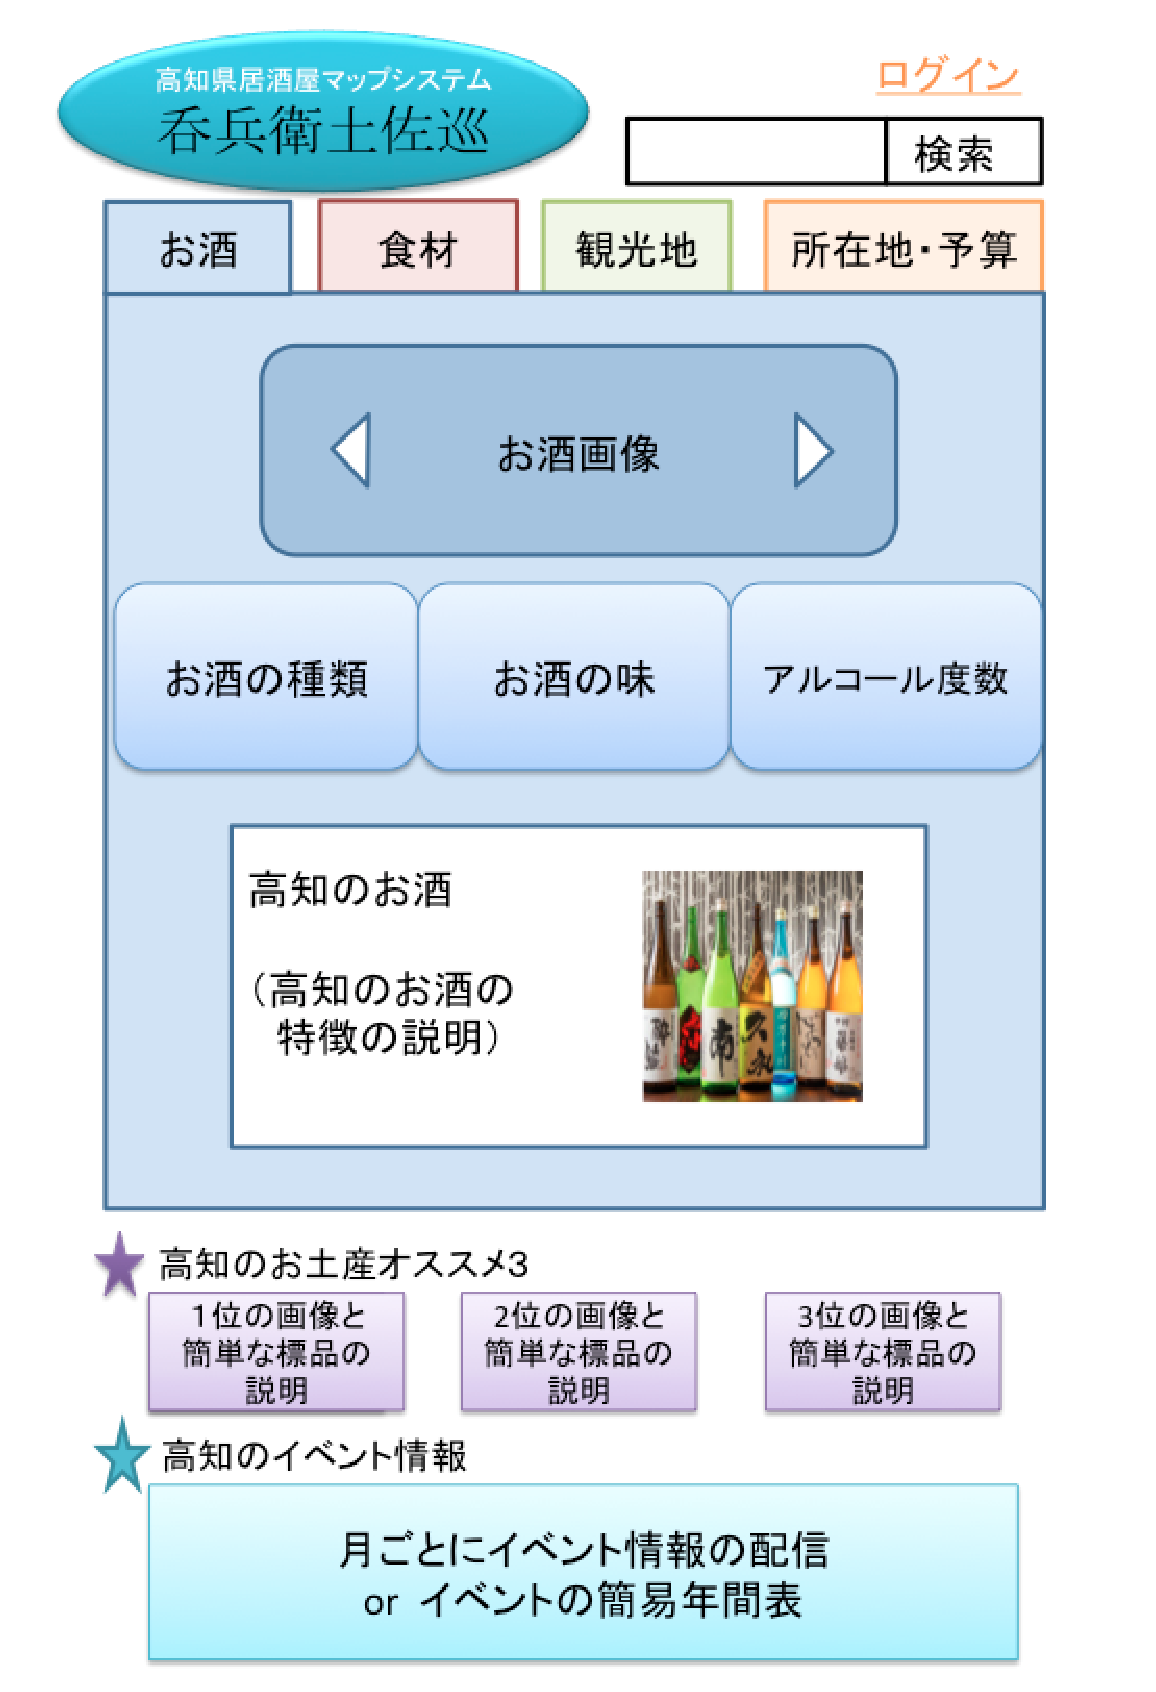
\includegraphics [height=11cm, width=10cm]{extrnal_design_document_image/1.eps}
    \caption {お酒から居酒屋を検索する画面}
    \label {fig:1}
    \end{center}
\end {figure}

検索項目
\begin{enumerate}
\item お酒の種類
お酒の種類から居酒屋を検索できます(図\ref{fig:2})。

\begin {figure}[htbp]
    \begin{center}
    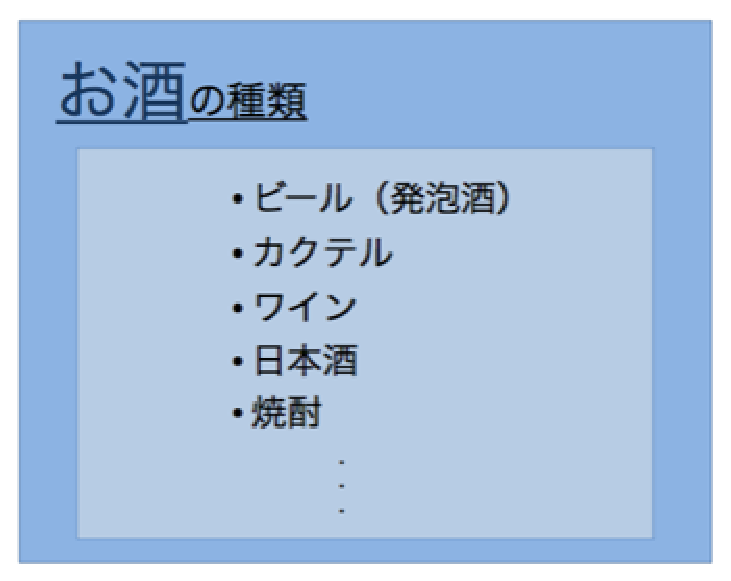
\includegraphics [height=7cm, width=7cm]{extrnal_design_document_image/2.eps}
    \caption {お酒の種類を表示した画面}
    \label {fig:2}
    \end{center}
\end {figure}

\item お酒の銘柄
お酒の種類からお酒の銘柄に遷移することができ、お酒の銘柄から居酒屋を検索することができます(図\ref{fig:3})。

\begin {figure}[htbp]
    \begin{center}
    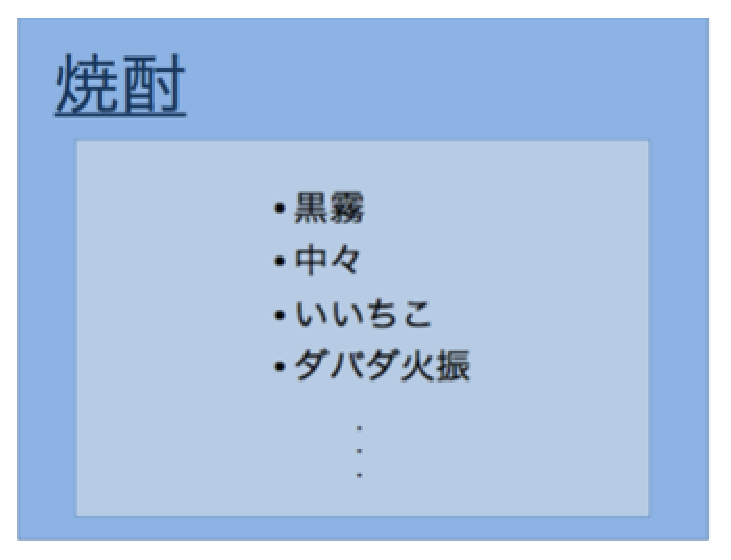
\includegraphics [height=7cm, width=7cm]{extrnal_design_document_image/3.eps}
    \caption {選択した種類に当てはまる酒名(銘柄)を表示した画面}
    \label {fig:3}
    \end{center}
\end {figure}


\item お酒の味
お酒の味(甘さ、辛さ、渋さなど)から居酒屋を検索することができます(図\ref{fig:4})。

\begin {figure}[htbp]
    \begin{center}
    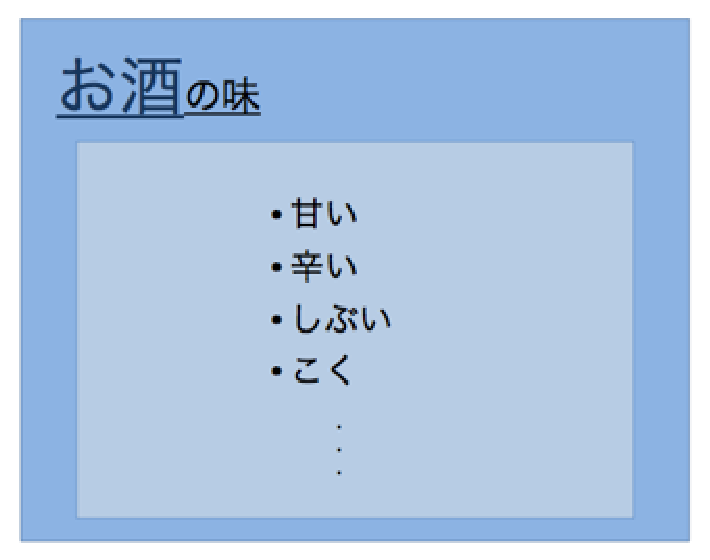
\includegraphics [height=7cm, width=7cm]{extrnal_design_document_image/4.eps}
    \caption {お酒の味が表示される画面}
    \label {fig:4}
    \end{center}
\end {figure}

\item アルコール度数
アルコール度数から居酒屋を検索することができます(図\ref{fig:5})。

\begin {figure}[htbp]
    \begin{center}
    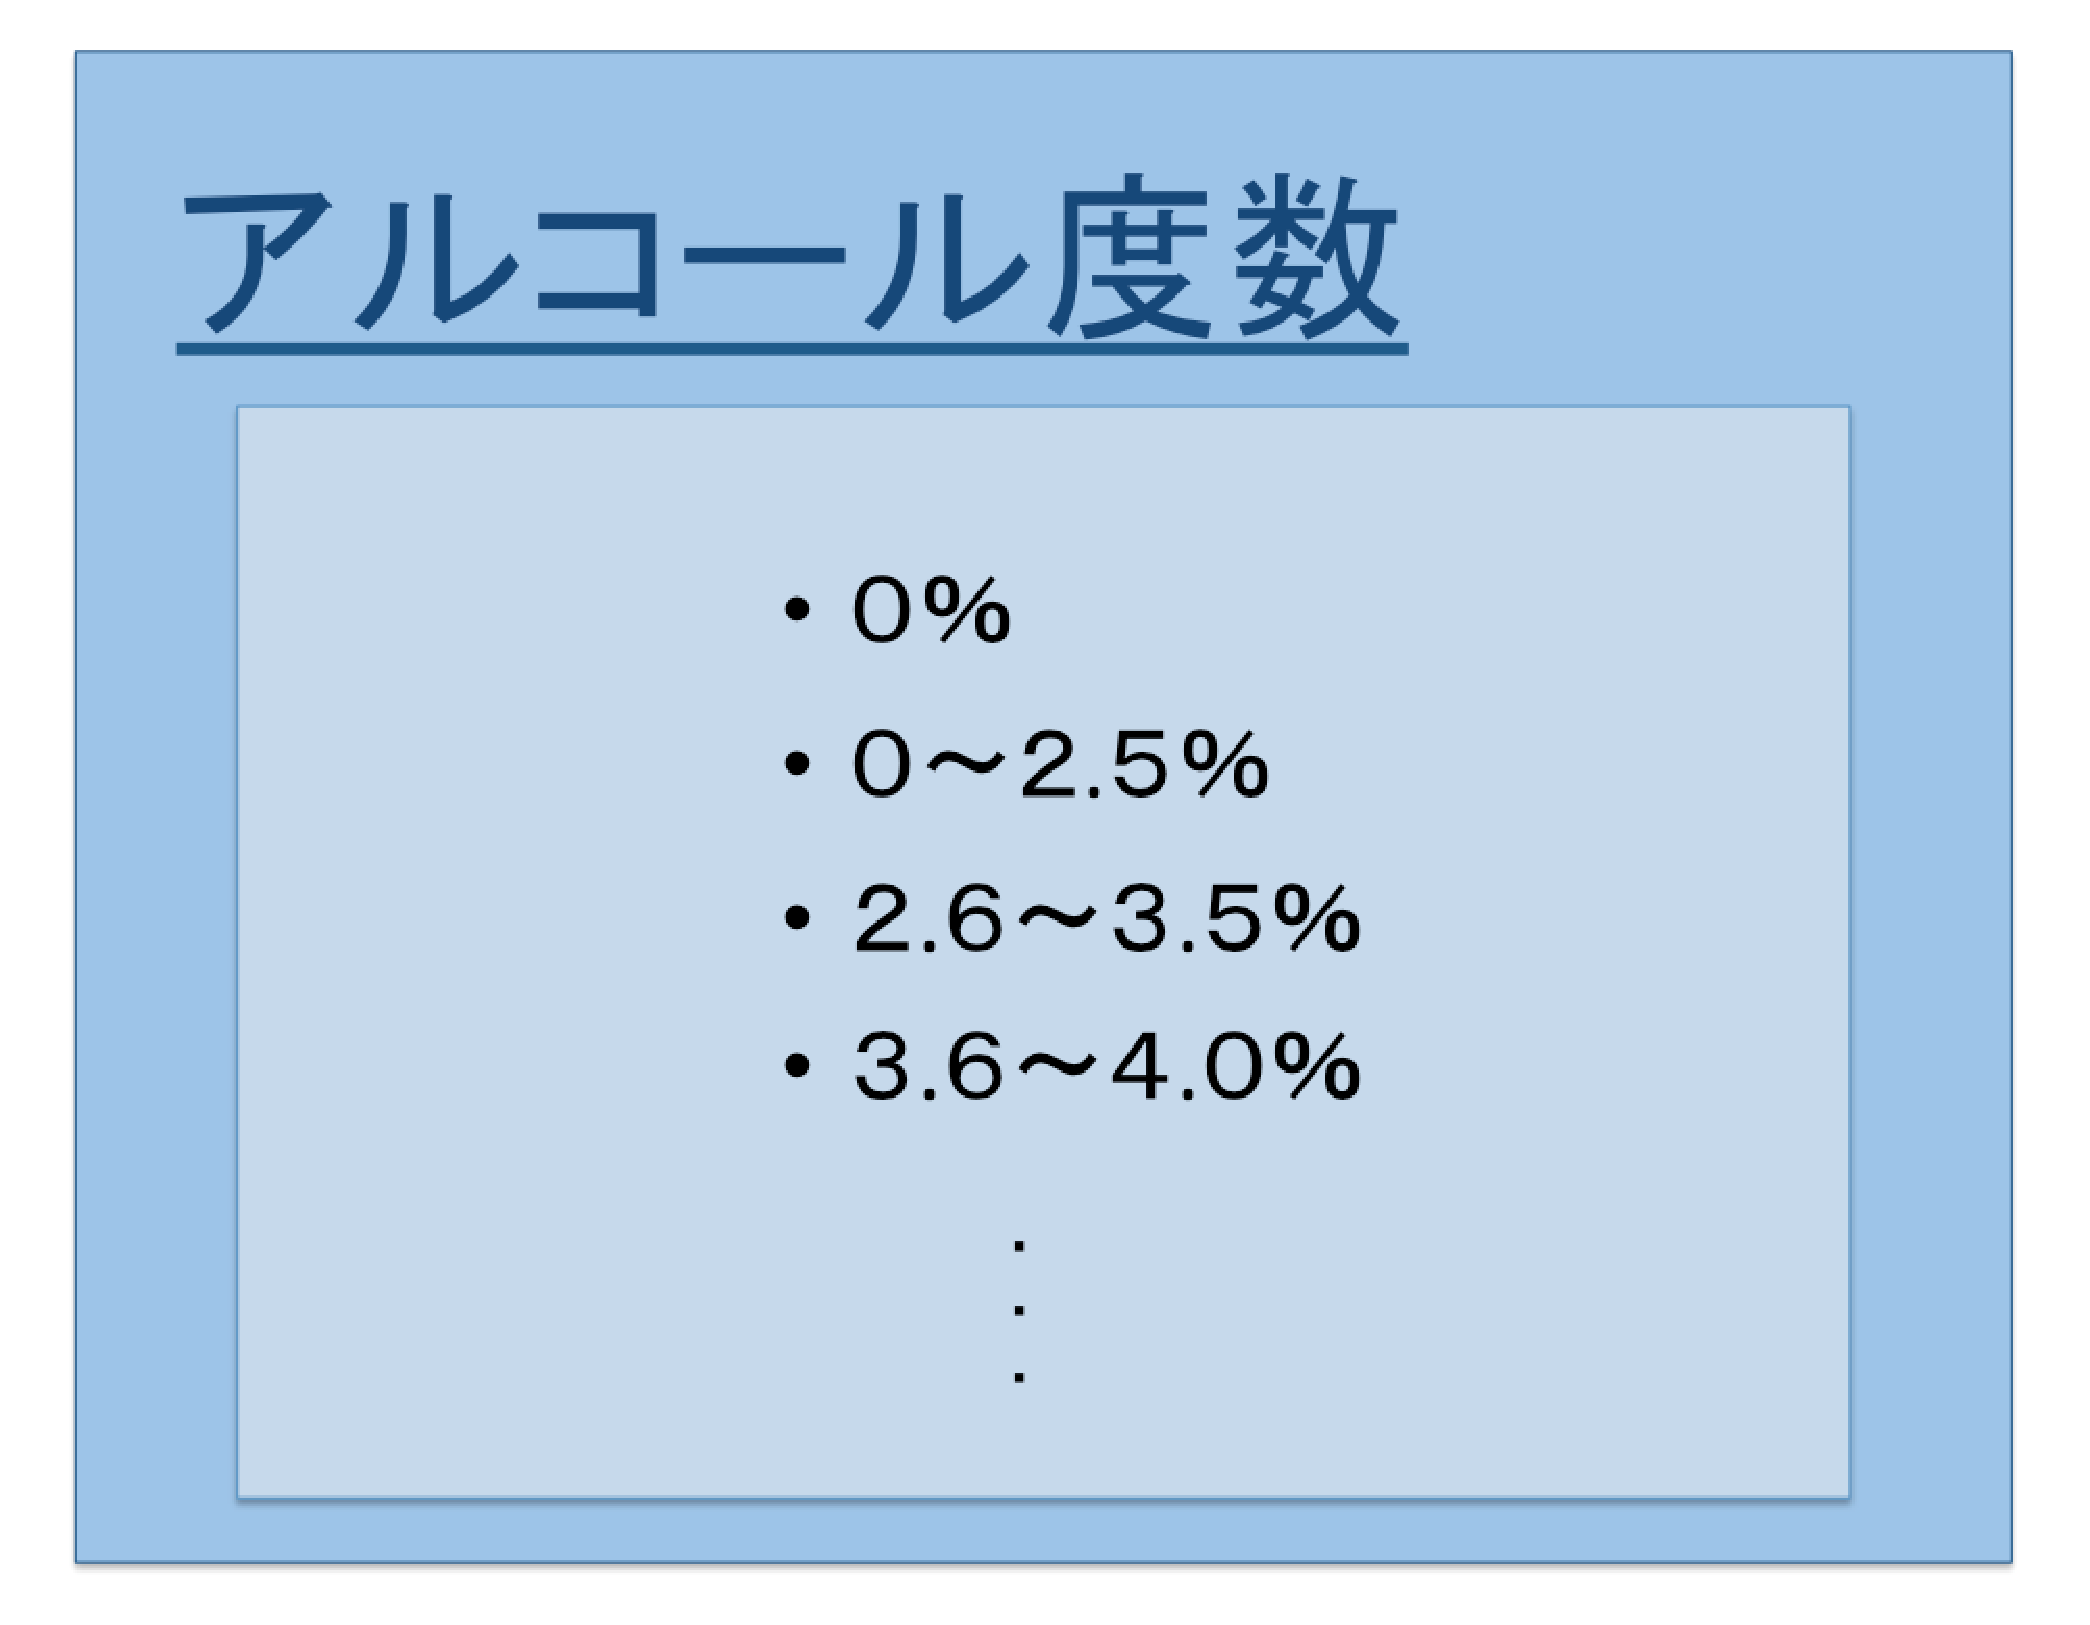
\includegraphics [height=7cm, width=7cm]{extrnal_design_document_image/5.eps}
    \caption {アルコール度数が表示される画面}
    \label {fig:5}
    \end{center}
\end {figure}

\end{enumerate}

\begin{enumerate}
\item [入力] 検索条件(複数入力可)
\item [出力] 検索条件に合ったお酒の一覧
\item [処理] 検索条件に合ったお酒をデータベースから取り出します
\end{enumerate}


\subsection{食材および郷土料理から店舗を検索する機能}
これは、高知県の食材や郷土料理から、それらを取り扱っている店舗を検索する機能です。
ユーザには、高知県の食材や郷土料理から居酒屋を検索する画面(図\ref{fig:6})が表示されます。
ユーザは高知県の食材から居酒屋を検索することができ(図\ref{fig:7})、各食材においての情報も閲覧することができます(図\ref{fig:8})。

\begin {figure}[htbp]
    \begin{center}
    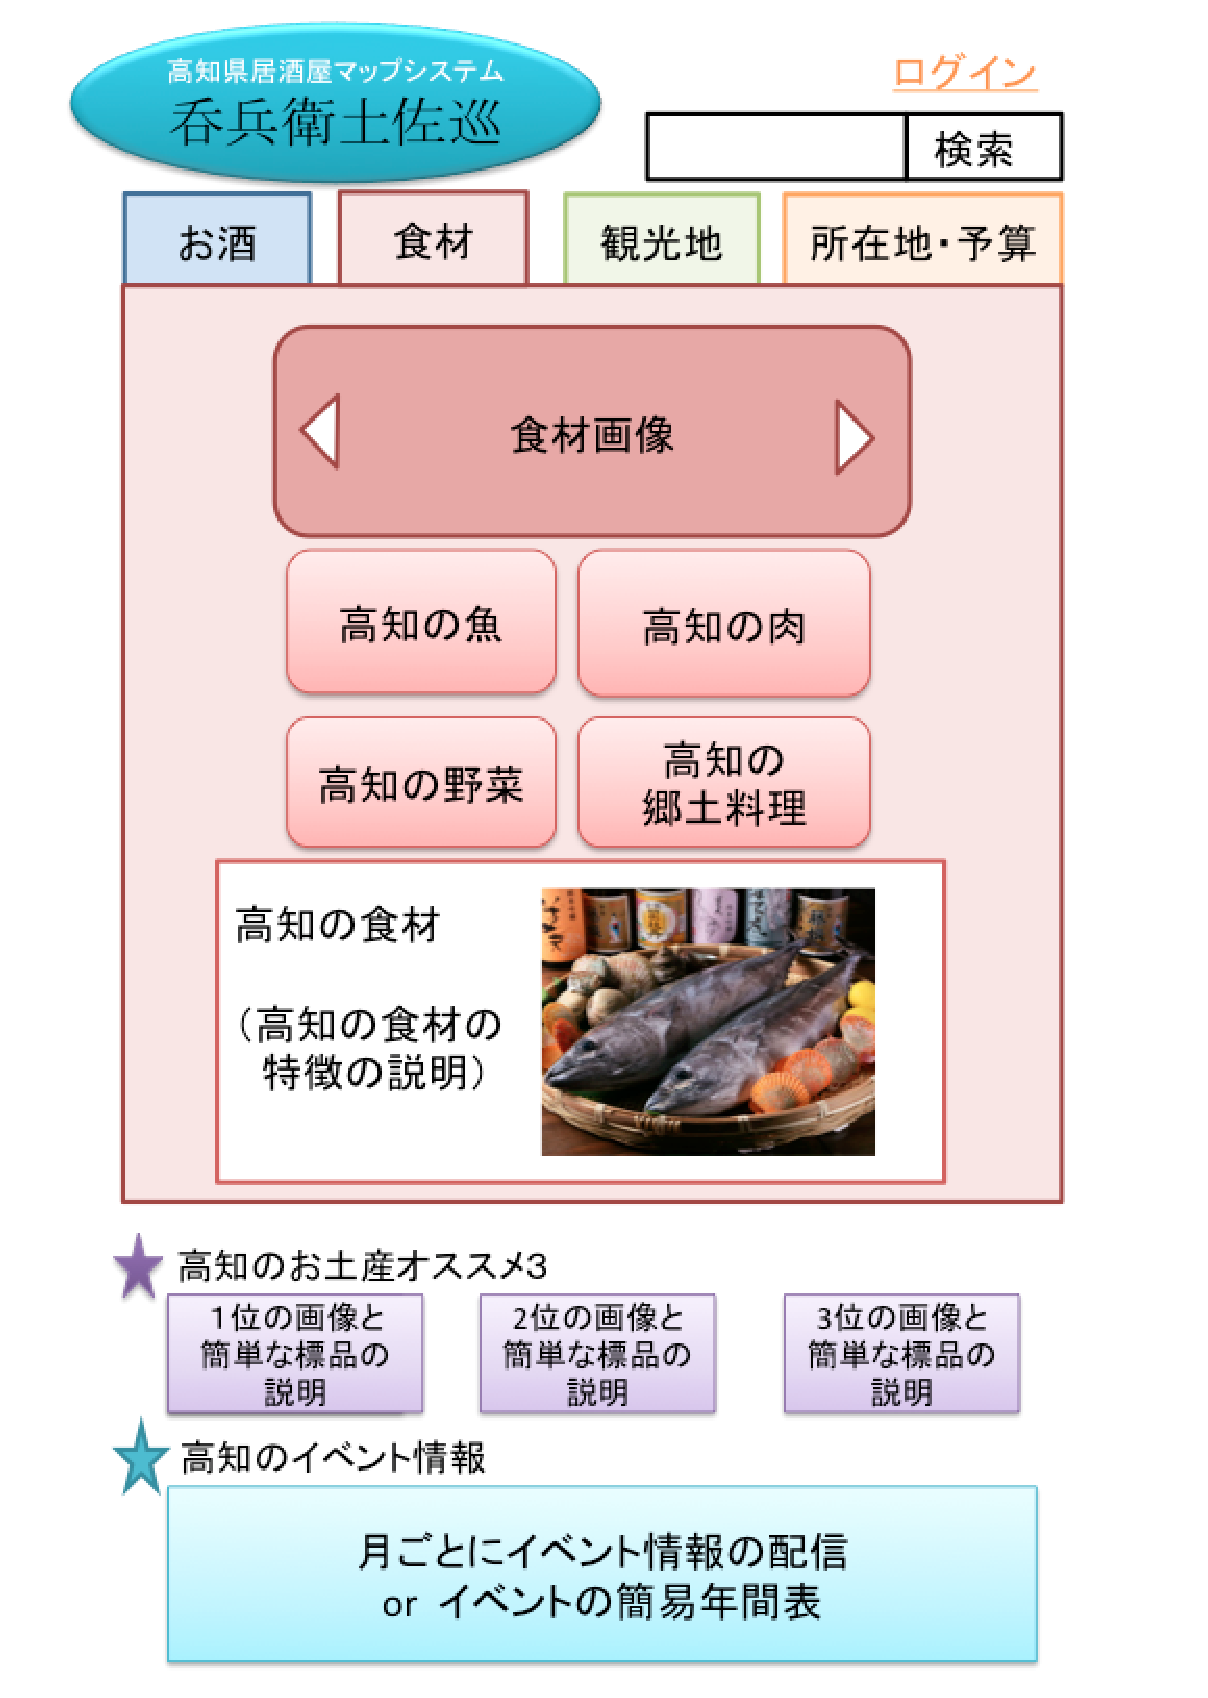
\includegraphics [height=12cm, width=10cm]{extrnal_design_document_image/6.eps}
    \caption {高知の食材および郷土料理から居酒屋を検索する画面}
    \label {fig:6}
    \end{center}
\end {figure}

\begin {figure}[htbp]
    \begin{center}
    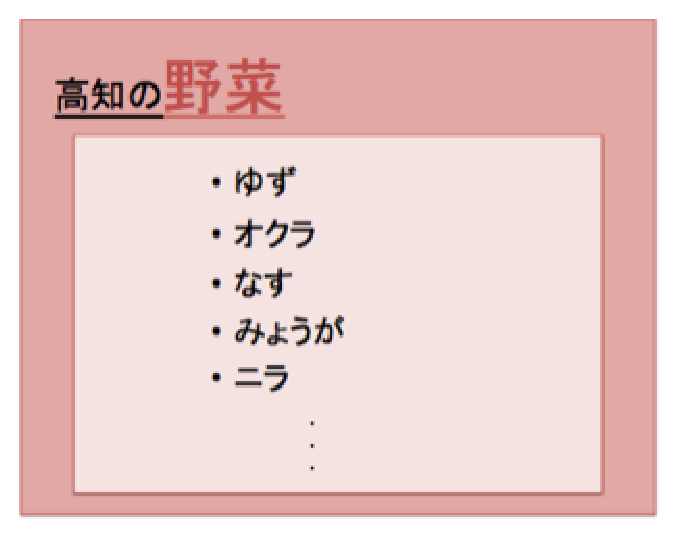
\includegraphics [height=7cm, width=7cm]{extrnal_design_document_image/7.eps}
    \caption {高知県の食材を表示する画面}
    \label {fig:7}
    \end{center}
\end {figure}

\begin {figure}[htbp]
    \begin{center}
    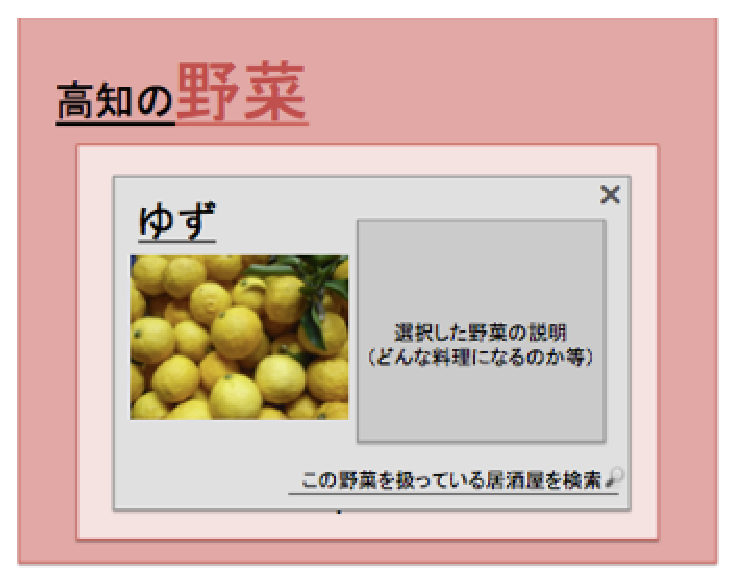
\includegraphics [height=7cm, width=7cm]{extrnal_design_document_image/8.eps}
      \caption {選択した食材の説明画面}
    \label {fig:8}
    \end{center}
\end {figure}

\begin{enumerate}
  \item [入力] 名産品
  \item [出力] 名産品を取り扱っている店舗の一覧
  \item [処理] 名産品を取り扱っている店舗をデータベースから取り出します
\end{enumerate}

\newpage
\subsection{観光地から店舗を検索する機能}
これは、高知県の観光地周辺に存在する店舗を検索する機能です。
ユーザには、高知県の観光地から居酒屋を検索する画面(図\ref{fig:9})が表示されます。
ユーザは高知県の観光地周辺の居酒屋を検索することができ(図\ref{fig:10})、各観光地においての情報も閲覧することができます(図\ref{fig:11})。

\begin {figure}[htpb]
    \begin{center}
    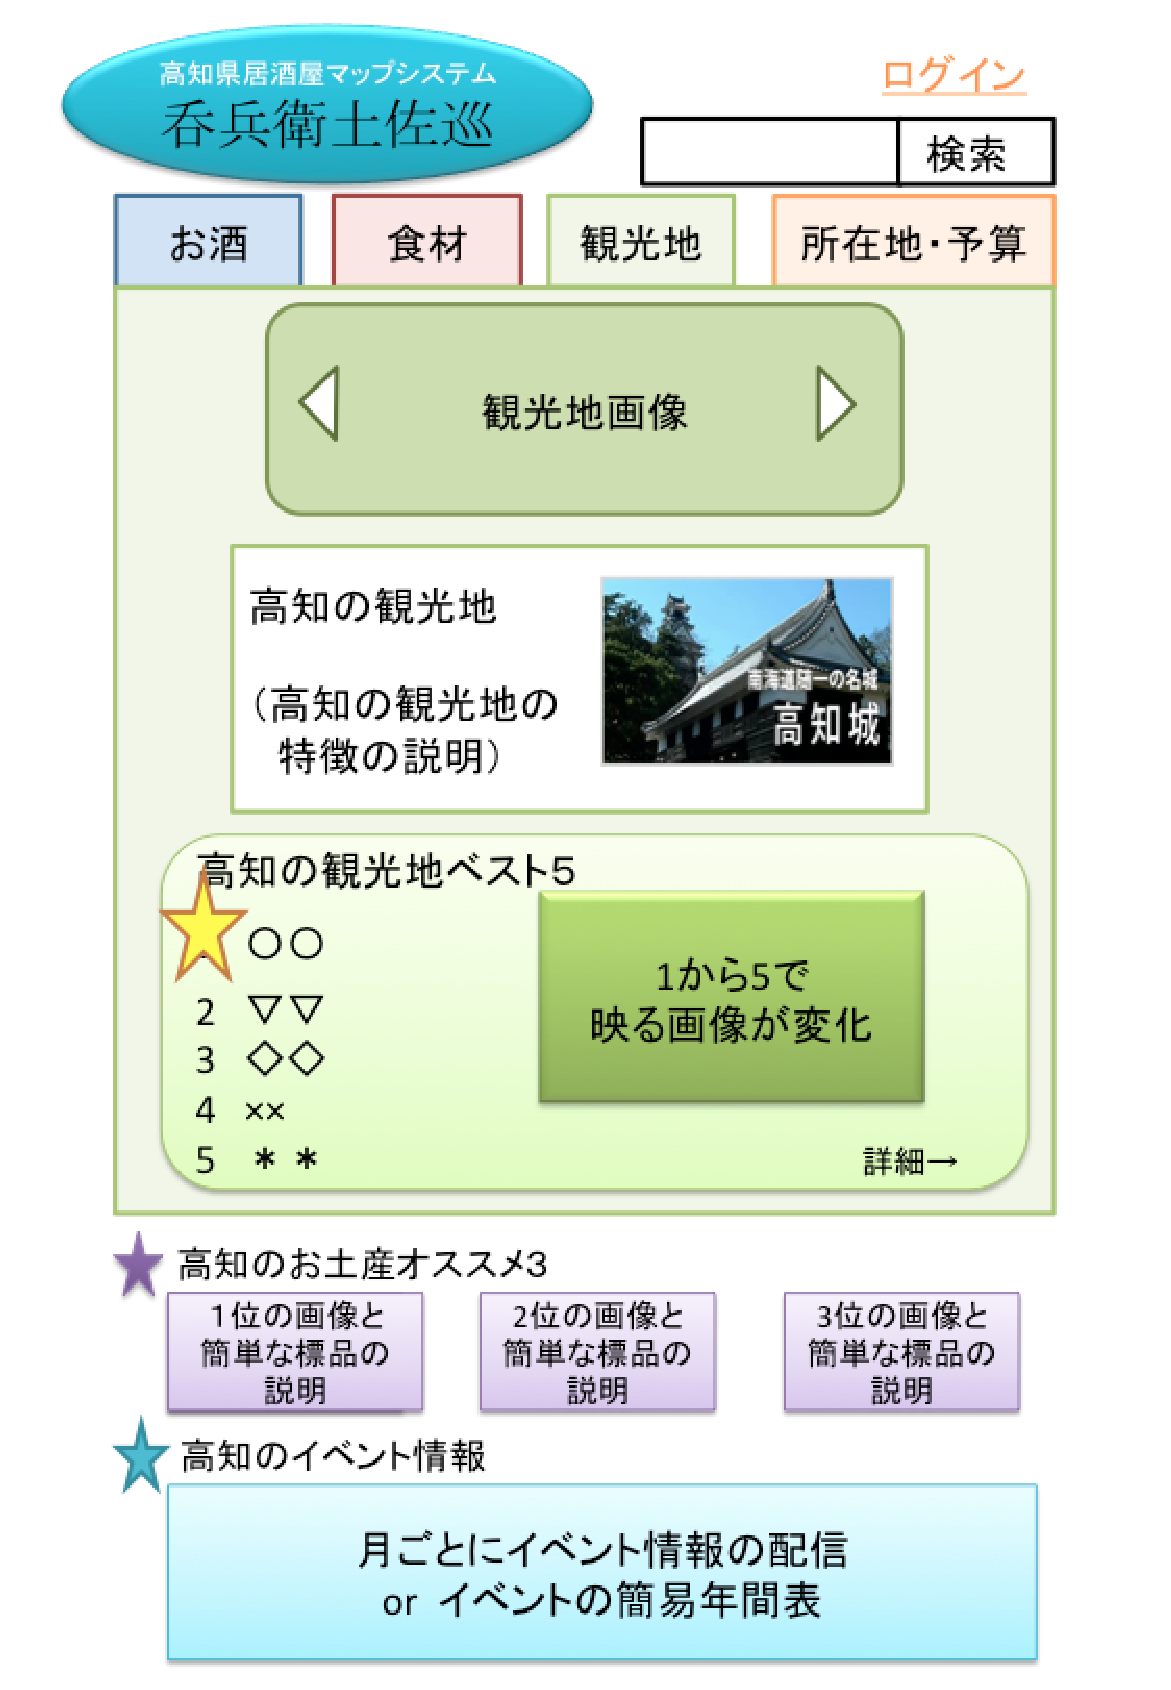
\includegraphics [height=12cm, width=10cm]{extrnal_design_document_image/9.eps}
    \caption {観光地から居酒屋を検索する画面}
    \label {fig:9}
    \end{center}
\end {figure}

\begin {figure}[htpb]
    \begin{center}
    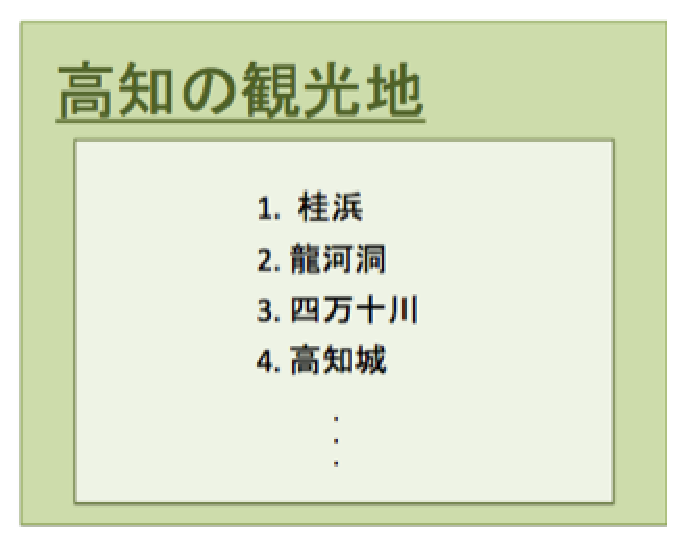
\includegraphics [height=7cm, width=7cm]{extrnal_design_document_image/10.eps}
    \caption {全ての観光地を表示する画面}
    \label {fig:10}
    \end{center}
\end {figure}

\begin {figure}[htbp]
    \begin{center}
    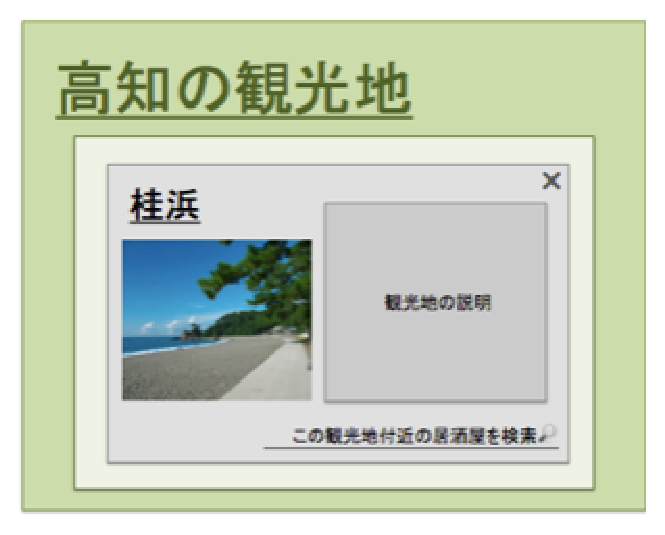
\includegraphics [height=7cm, width=7cm]{extrnal_design_document_image/11.eps}
    \caption {選択した観光地の説明画面}
    \label {fig:11}
    \end{center}
\end {figure}

\begin{enumerate}
  \item [入力] 観光地名
  \item [出力] 観光地付近に存在する店舗の一覧
  \item [処理] 観光地付近に存在する店舗をデータベースから取り出します
\end{enumerate}

\newpage
\subsection{その他の店舗情報から店舗を検索する機能}
これは、お酒、食材や郷土料理、観光地以外の下記の検索項目から店舗を検索する機能です。
ユーザには、様々な店舗情報から居酒屋を検索する画面(図\ref{fig:12})が表示されます。

\begin {figure}[htbp]
    \begin{center}
    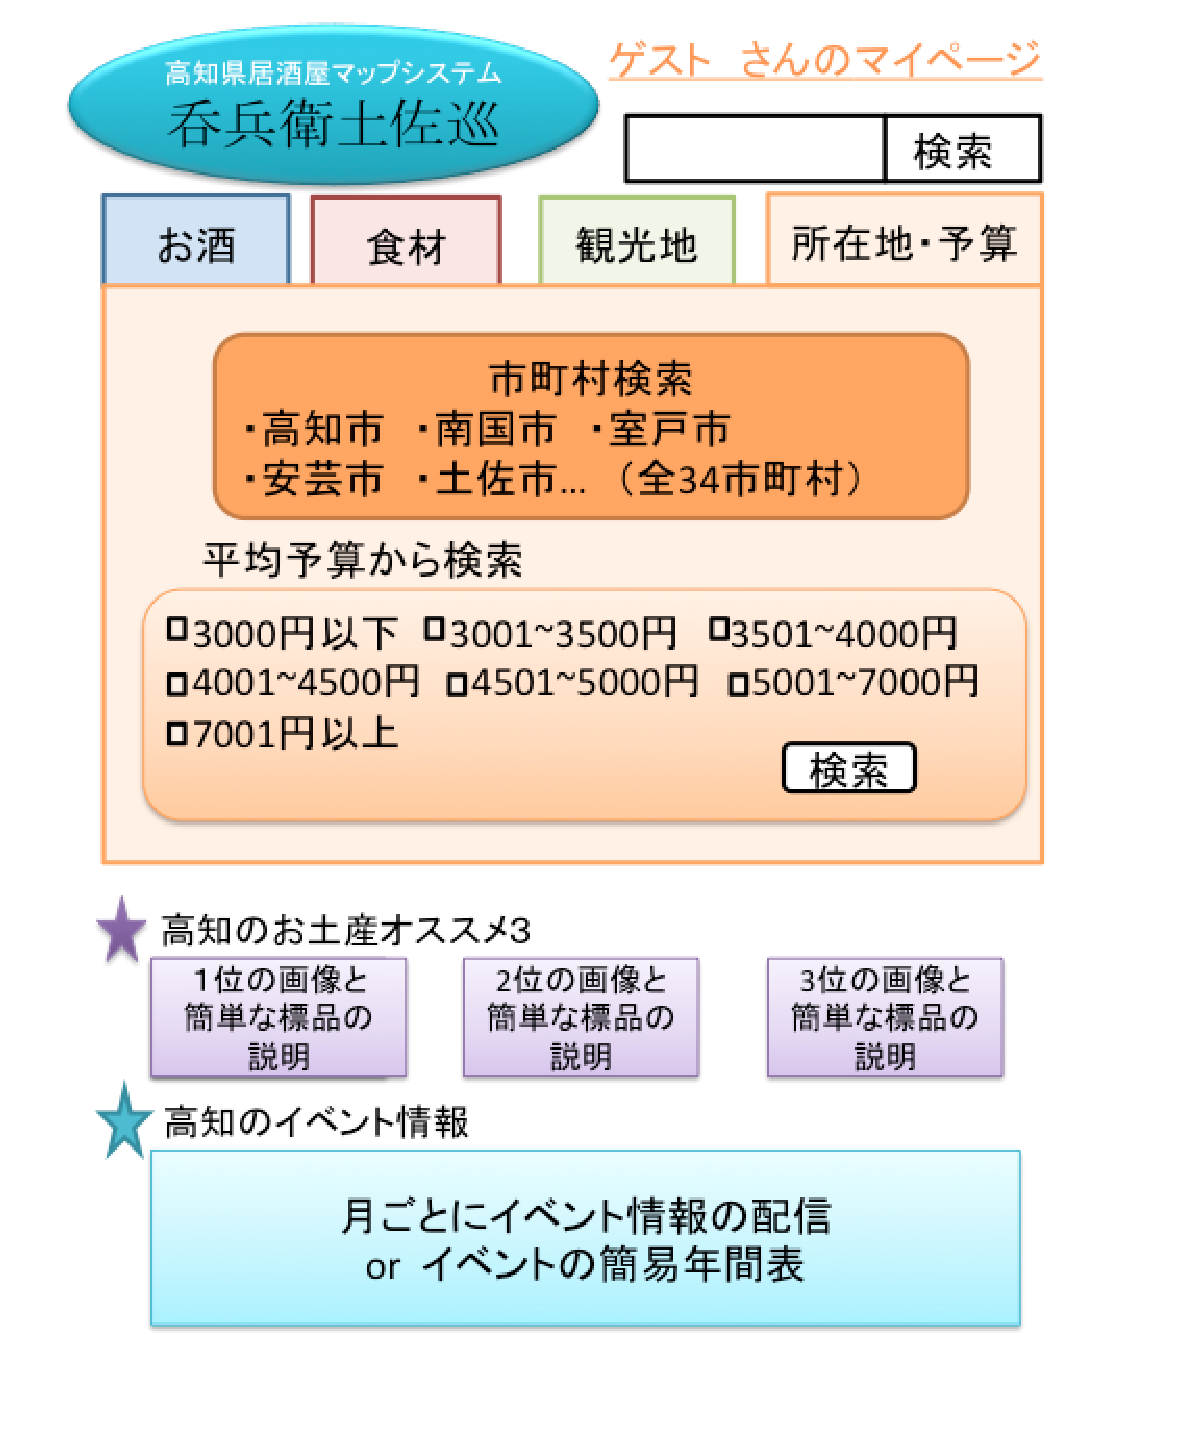
\includegraphics [height=11cm, width=10cm]{extrnal_design_document_image/12.eps}
    \caption {店舗の特徴から居酒屋を検索する画面}
    \label {fig:12}
    \end{center}
\end {figure}


検索項目
\begin{enumerate}
\item 店舗名
検索欄で店舗名を入力することで、目的の居酒屋を検索できます。

\item 住所
店舗の住所から居酒屋を検索できます。図\ref{fig:12}の市町村検索を活用することで、市町村から居酒屋を割り出すことができます(図\ref{fig:13})。

\begin {figure}[htbp]
    \begin{center}
    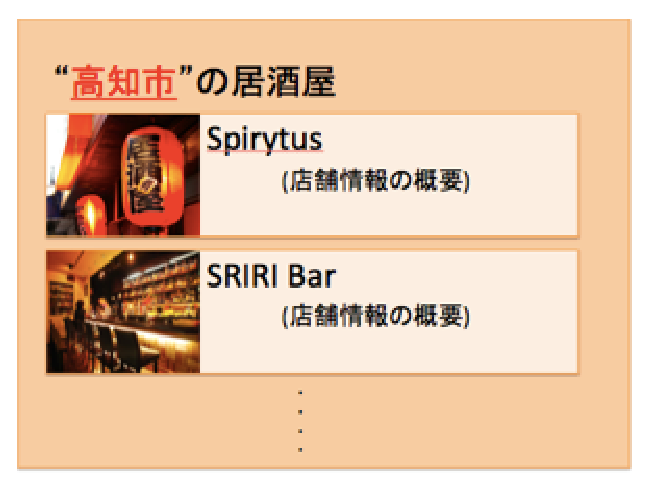
\includegraphics [height=7cm, width=7cm]{extrnal_design_document_image/13.eps}
      \caption {選択した市町村に所在する居酒屋の一覧表を表示する画面}
    \label {fig:13}
    \end{center}
\end {figure}

\item 平均予算
店舗で消費する平均予算から居酒屋を検索できます。検索結果は図\ref{fig:13}と同様の画面が表示されます。


\item 宴会が行なえるかどうか
宴会が行えるか否かで居酒屋を検索することができます。検索結果は図\ref{fig:13}と同様の画面が表示されます。

\end{enumerate}

\begin{enumerate}
\item [入力] 検索条件(複数入力可)
\item [出力] 検索条件に合った店舗の一覧
\item [処理] 検索条件に合った店舗をデータベースから取り出します
\end{enumerate}


\subsection{新規ユーザ登録機能}
新規のユーザがアカウントを登録する機能です。

登録項目
\begin{enumerate}
  \item ユーザネーム
  \item e-mailアドレス
  \item パスワード
\end{enumerate}

\begin{enumerate}
  \item [入力] 登録項目
  \item [出力] マイページ
  \item [処理] 登録項目に沿ってアカウントを作成し、データベースに保存します
\end{enumerate}

\subsection{ユーザログイン機能}
ユーザがマイページにログインする機能です。

\begin{enumerate}
  \item [入力] ユーザネーム、パスワード
  \item [出力] マイページ
  \item [処理] ユーザネームとパスワードをもとに、データベースからアカウント情報を取り出します
\end{enumerate}
\subsection{店舗登録機能}
店舗側は端末を使用して店舗登録申請フォームにアクセスし、必要情報を入力し申請を行います。
この申請に対し運営者側で店舗の広告を行うか判断します。
広告を行うと判断された場合、e-mailアドレス、パスワードをデータベースに登録します。
このe-mailアドレス、パスワードを使用しログインすることでページ編集画面にアクセスし、店舗情報の編集を行います。

\subsubsection{店舗の申請機能}
\begin{enumerate}
\item[入力] e-mailアドレス
\item[出力] メール送信
\item[処理] 登録ページのURLが記載されたメールを店舗側に送信します。店舗側はURLにアクセスし新規の登録を行い、運営側で登録された情報に対し審査を行います。登録された情報に不備等がなければそのまま登録を行います。不備等がある場合、店舗に対してメールや電話で問い合わせを行います。
\end{enumerate}

\subsubsection{店側のログイン機能}
\begin{enumerate}
\item[入力] e-mailアドレス、パスワード
\item[出力] ログイン成功ならば店舗個別ページ
\item[処理] 入力情報とデータベースを照合しログインの合否を判定します。ログインに成功した場合、店舗情報の編集画面に遷移します。
\end{enumerate}

\subsection{お酒のレビュー}
お酒の詳細情報画面(図\ref{fig:14})にお酒のレビュー項目を設けています。
内容としては、選択したお酒の味を十字のチャート図で評価します。
十字のチャート図においては二組の形容詞対を十字に対応させ、そのチャート図内で評価を行います(図\ref{fig:15})。
また、コメント入力欄を設け、お酒に対する味の感想やコメントを書くことができます。
さらに自身で書いたレビューや他人の書いたレビューを閲覧することができます(図\ref{fig:16})。

\begin {figure}[htbp]
    \begin{center}
    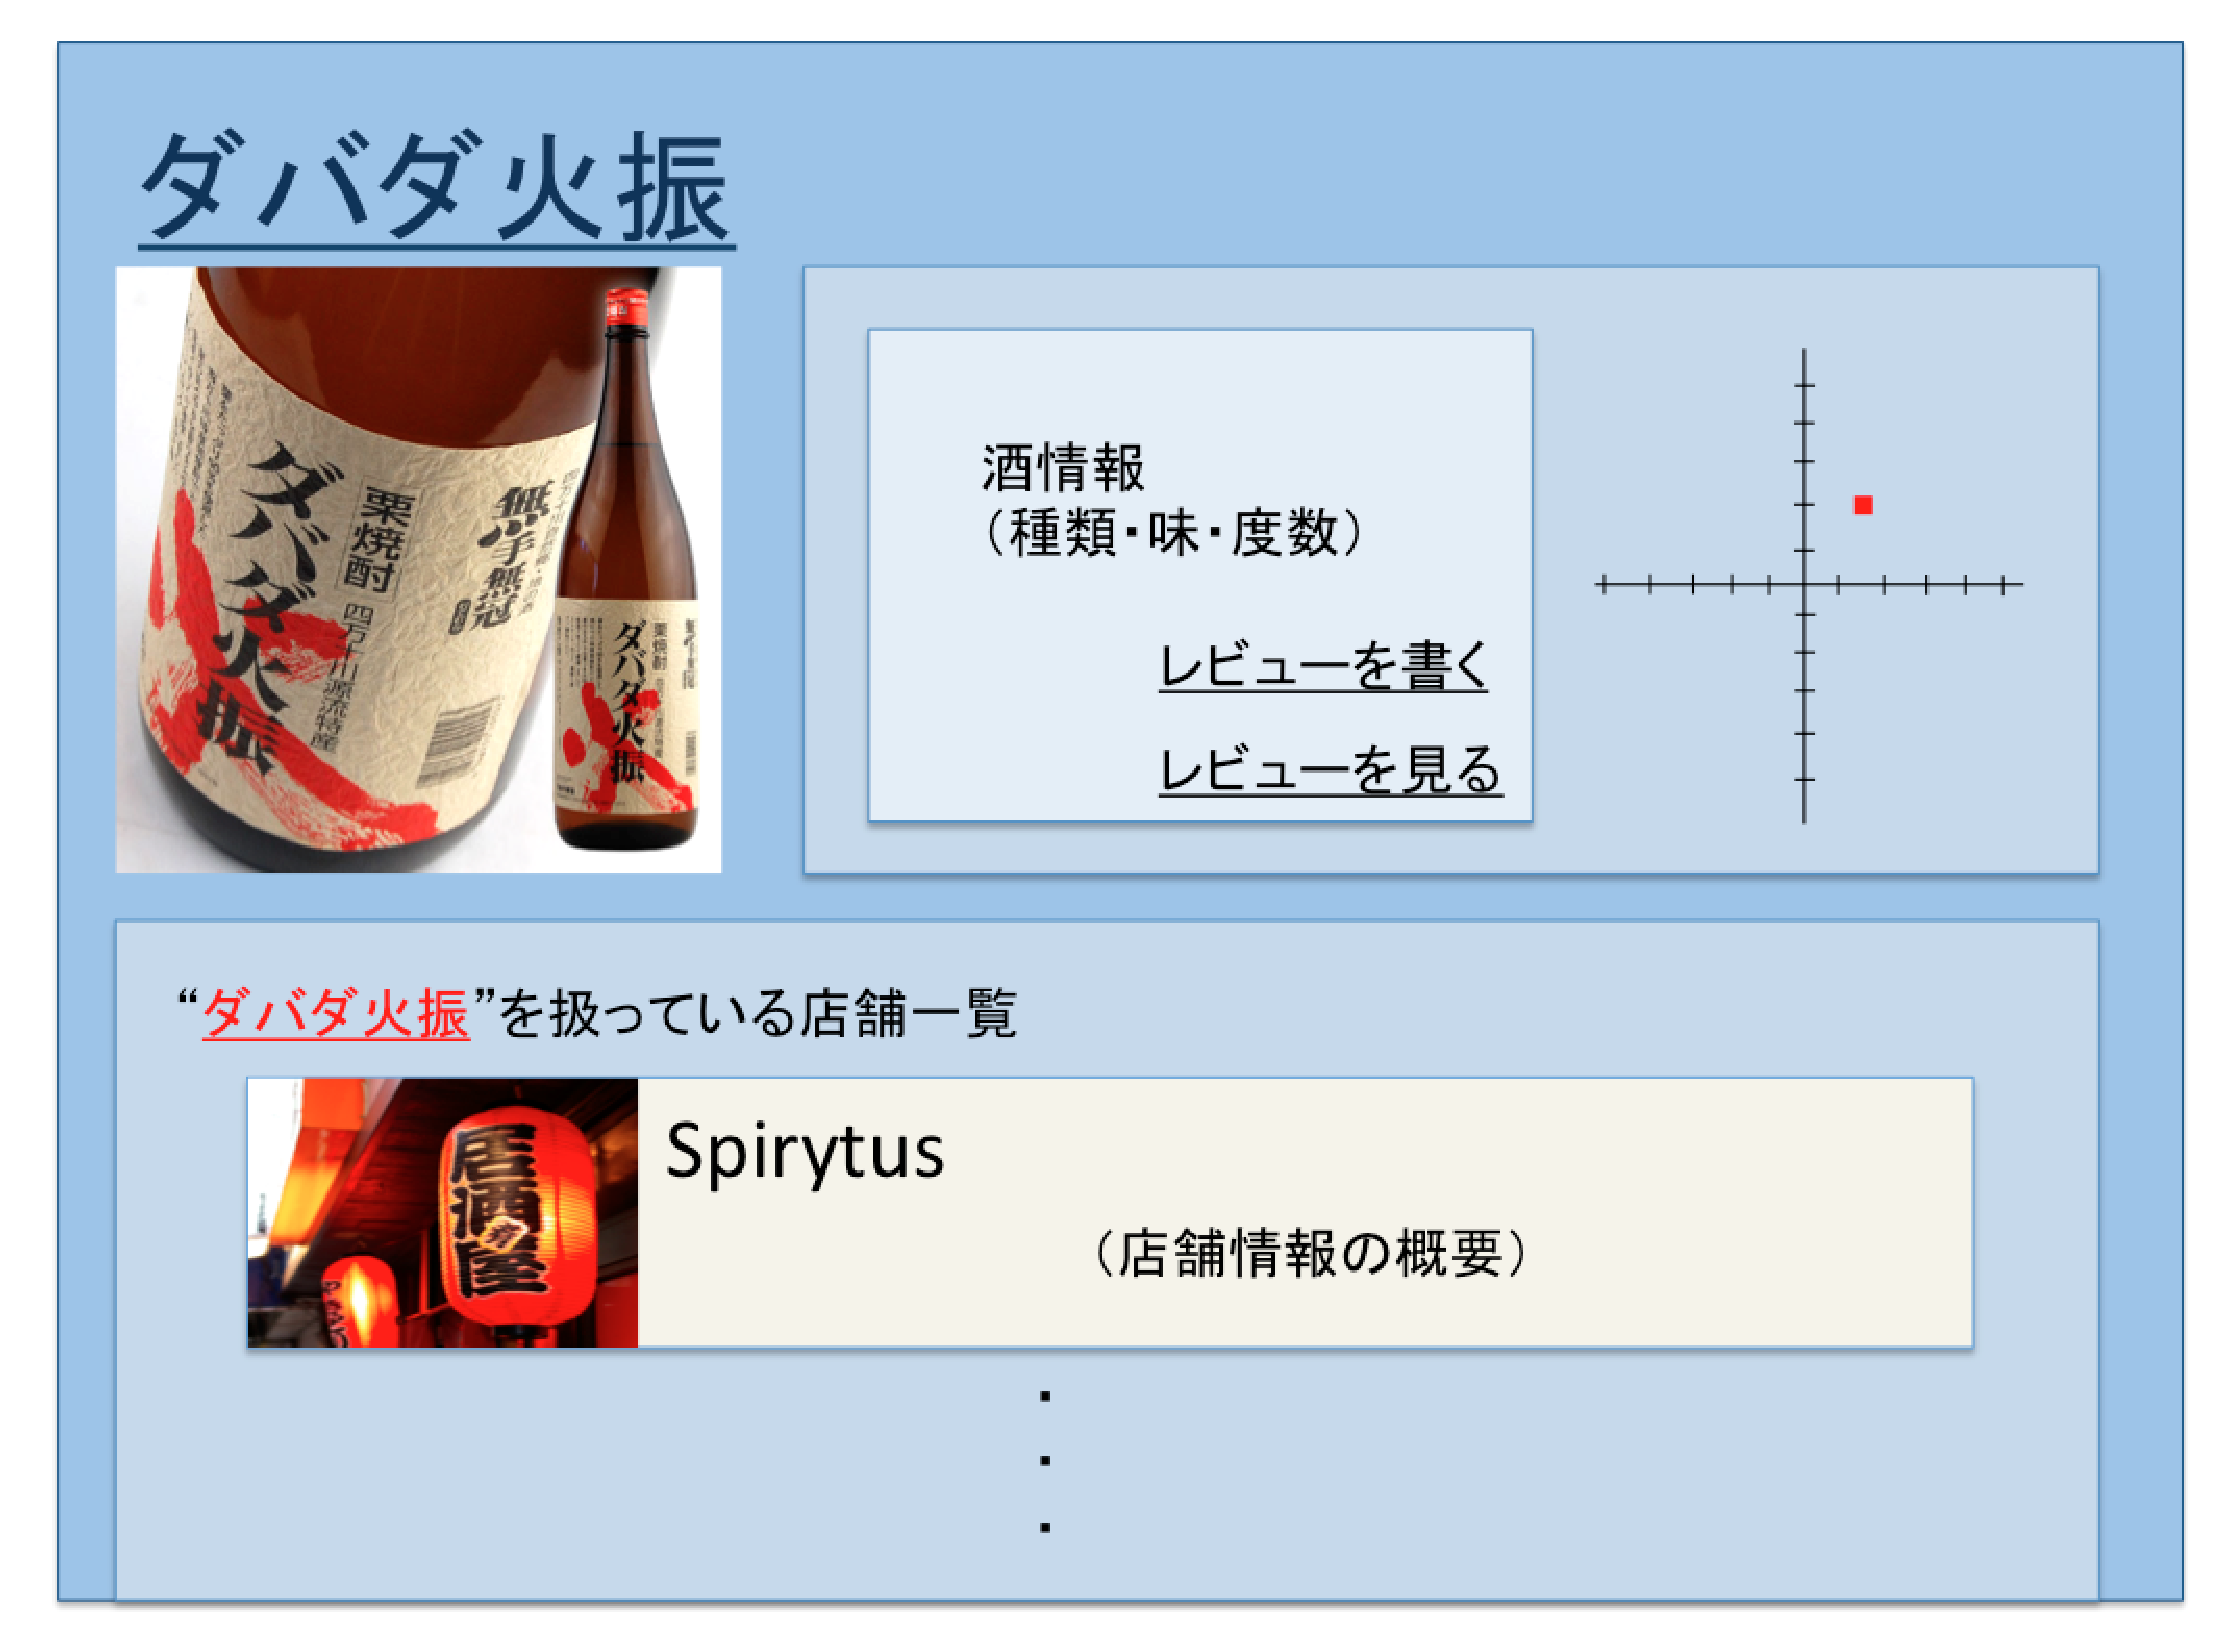
\includegraphics [height=7cm, width=7cm]{extrnal_design_document_image/14.eps}
    \caption {お酒の詳細情報およびそのお酒を扱っている店舗の一覧が表示される画面}
    \label {fig:14}
    \end{center}
\end {figure}

\begin {figure}[htbp]
    \begin{center}
    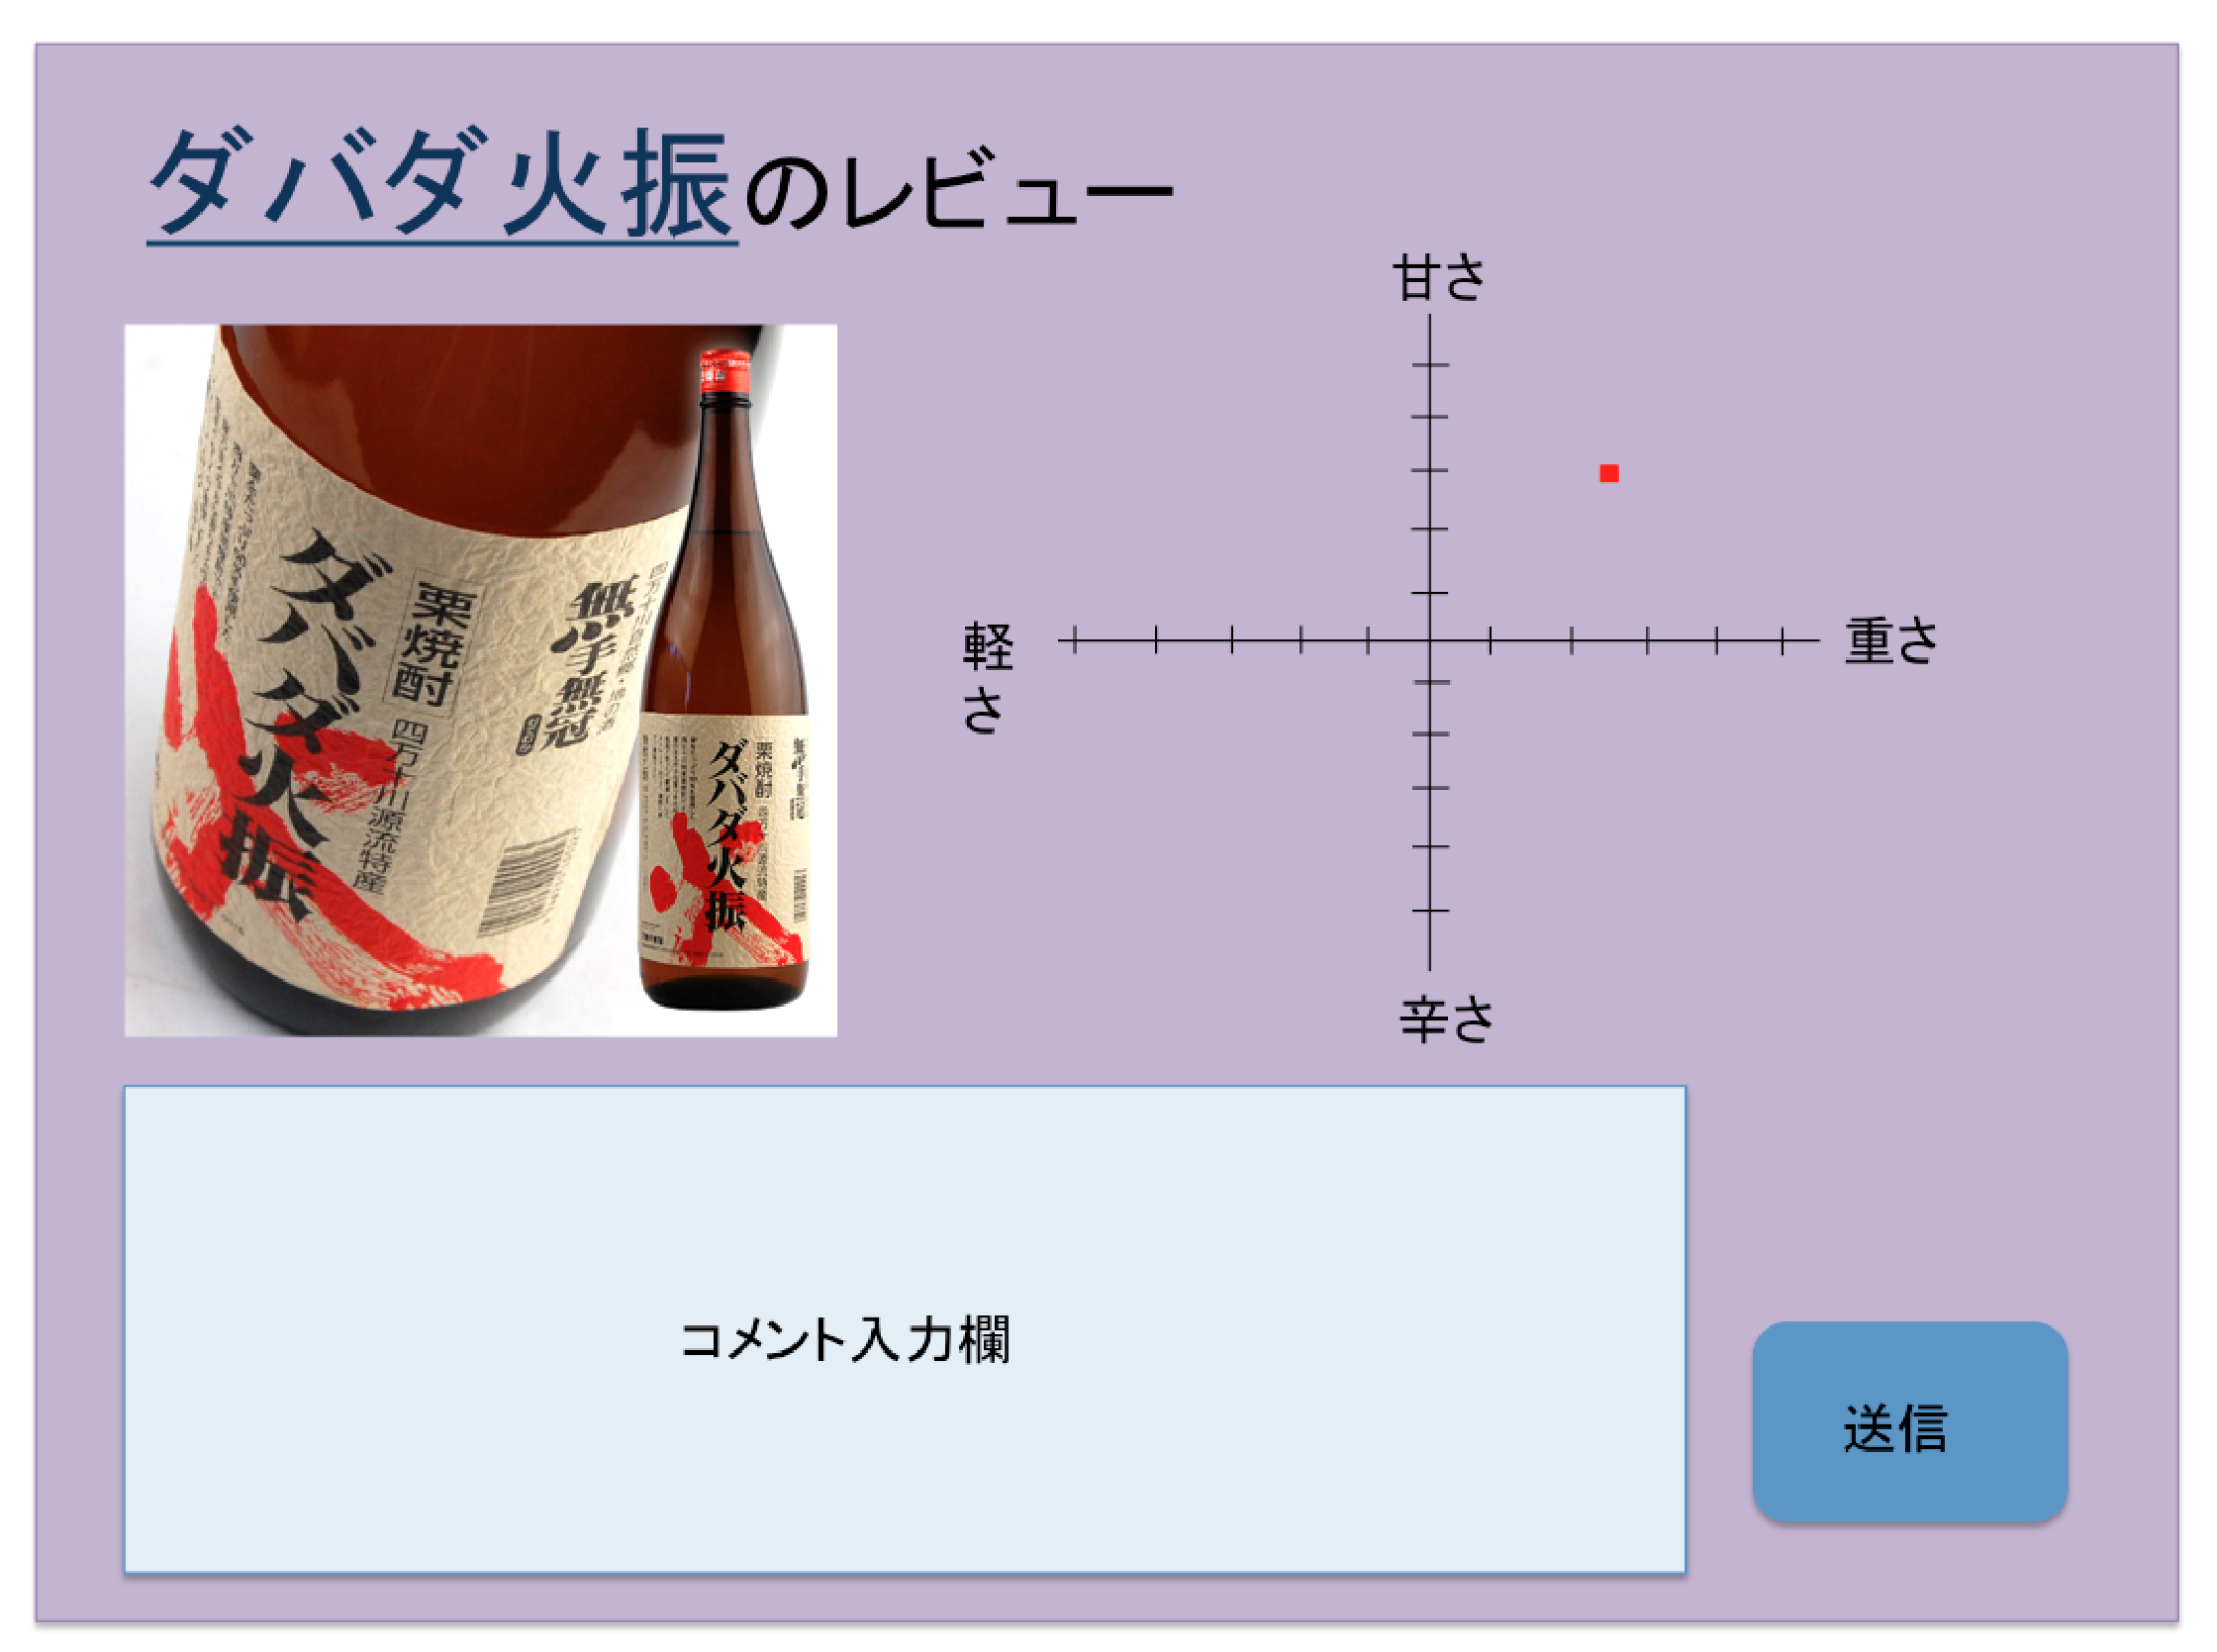
\includegraphics [height=7cm, width=7cm]{extrnal_design_document_image/15.eps}
    \caption {お酒のレビュー編集画面}
    \label {fig:15}
    \end{center}
\end {figure}

\begin {figure}[htbp]
    \begin{center}
    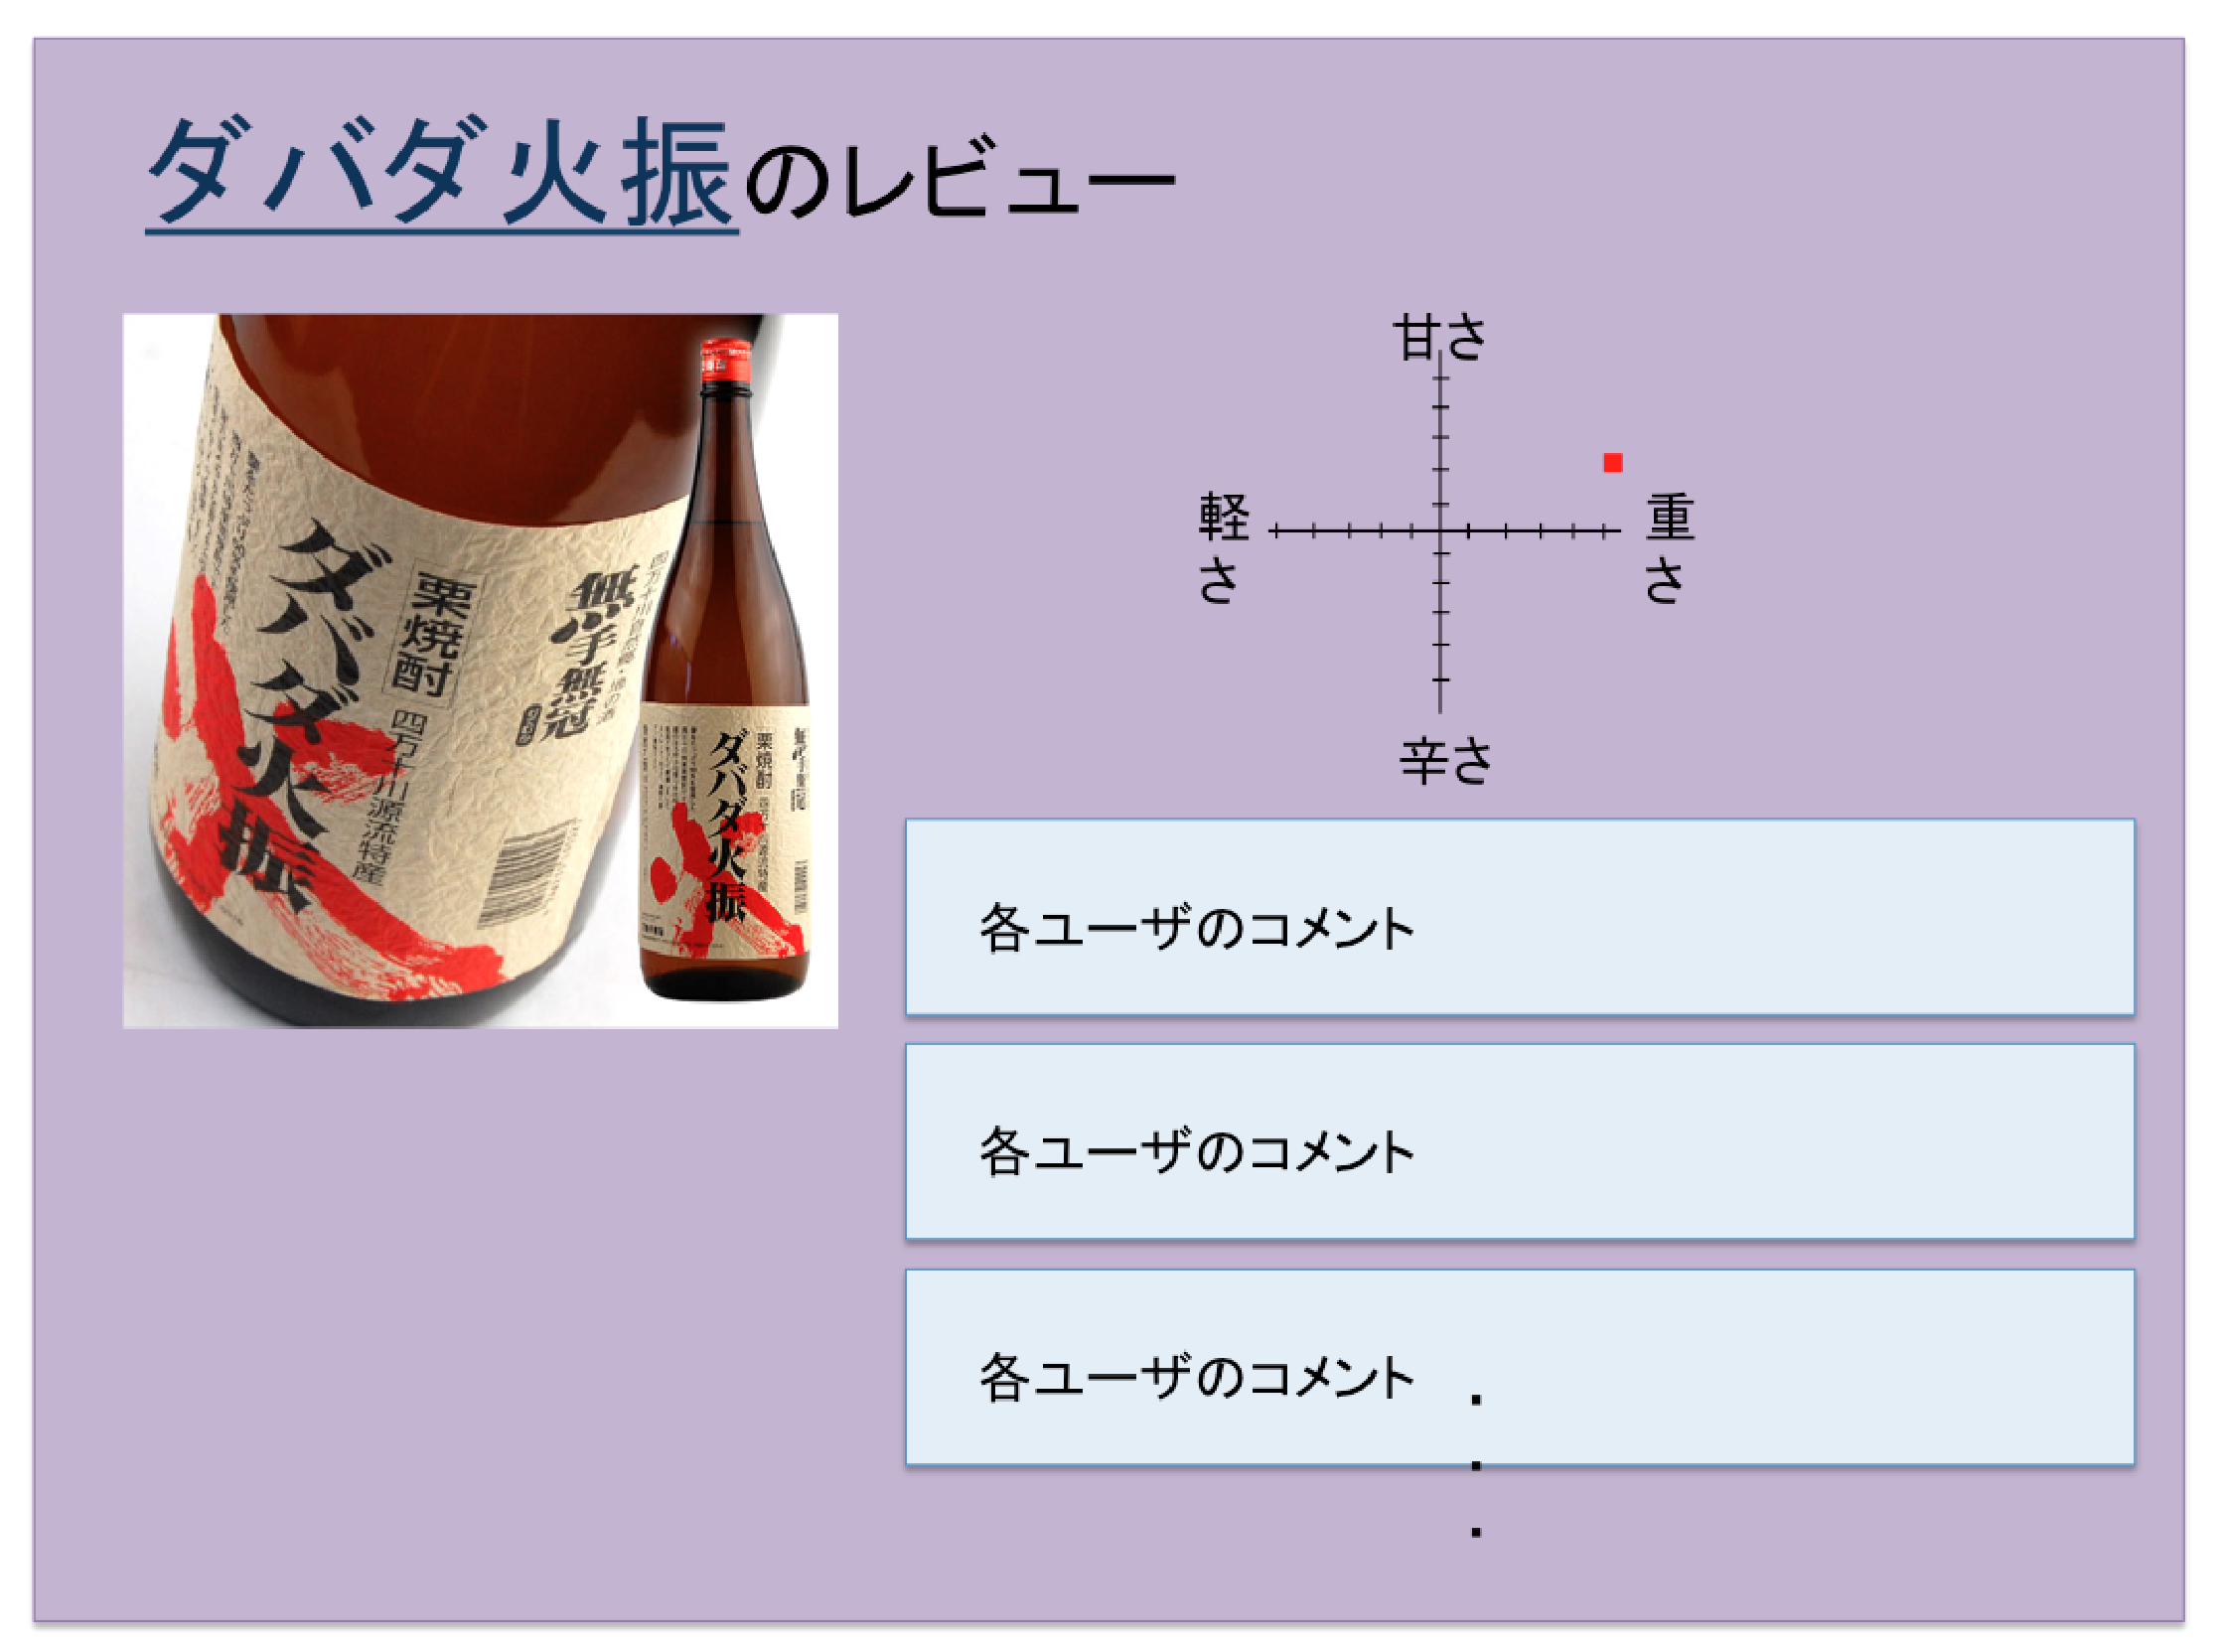
\includegraphics [height=7cm, width=7cm]{extrnal_design_document_image/16.eps}
    \caption {お酒のレビュー閲覧画面}
    \label {fig:16}
    \end{center}
\end {figure}


\subsection{店舗のレビュー}
店舗の詳細情報画面(図\ref{fig:17})に店舗のレビュー項目を設けています。
内容としては、選択した店舗の全体の雰囲気の良し悪しを0〜5の6段階の数値で評価します。
また、コメント入力欄を設け、店舗に来た感想やコメントを書くことができます。
さらに自身で書いたレビューや他人の書いたレビューを閲覧することができます。
店舗のレビュー編集および閲覧画面はお酒レビュー画面(図\ref{fig:15}、図\ref{fig:16})と同様です。

\begin {figure}[htbp]
    \begin{center}
    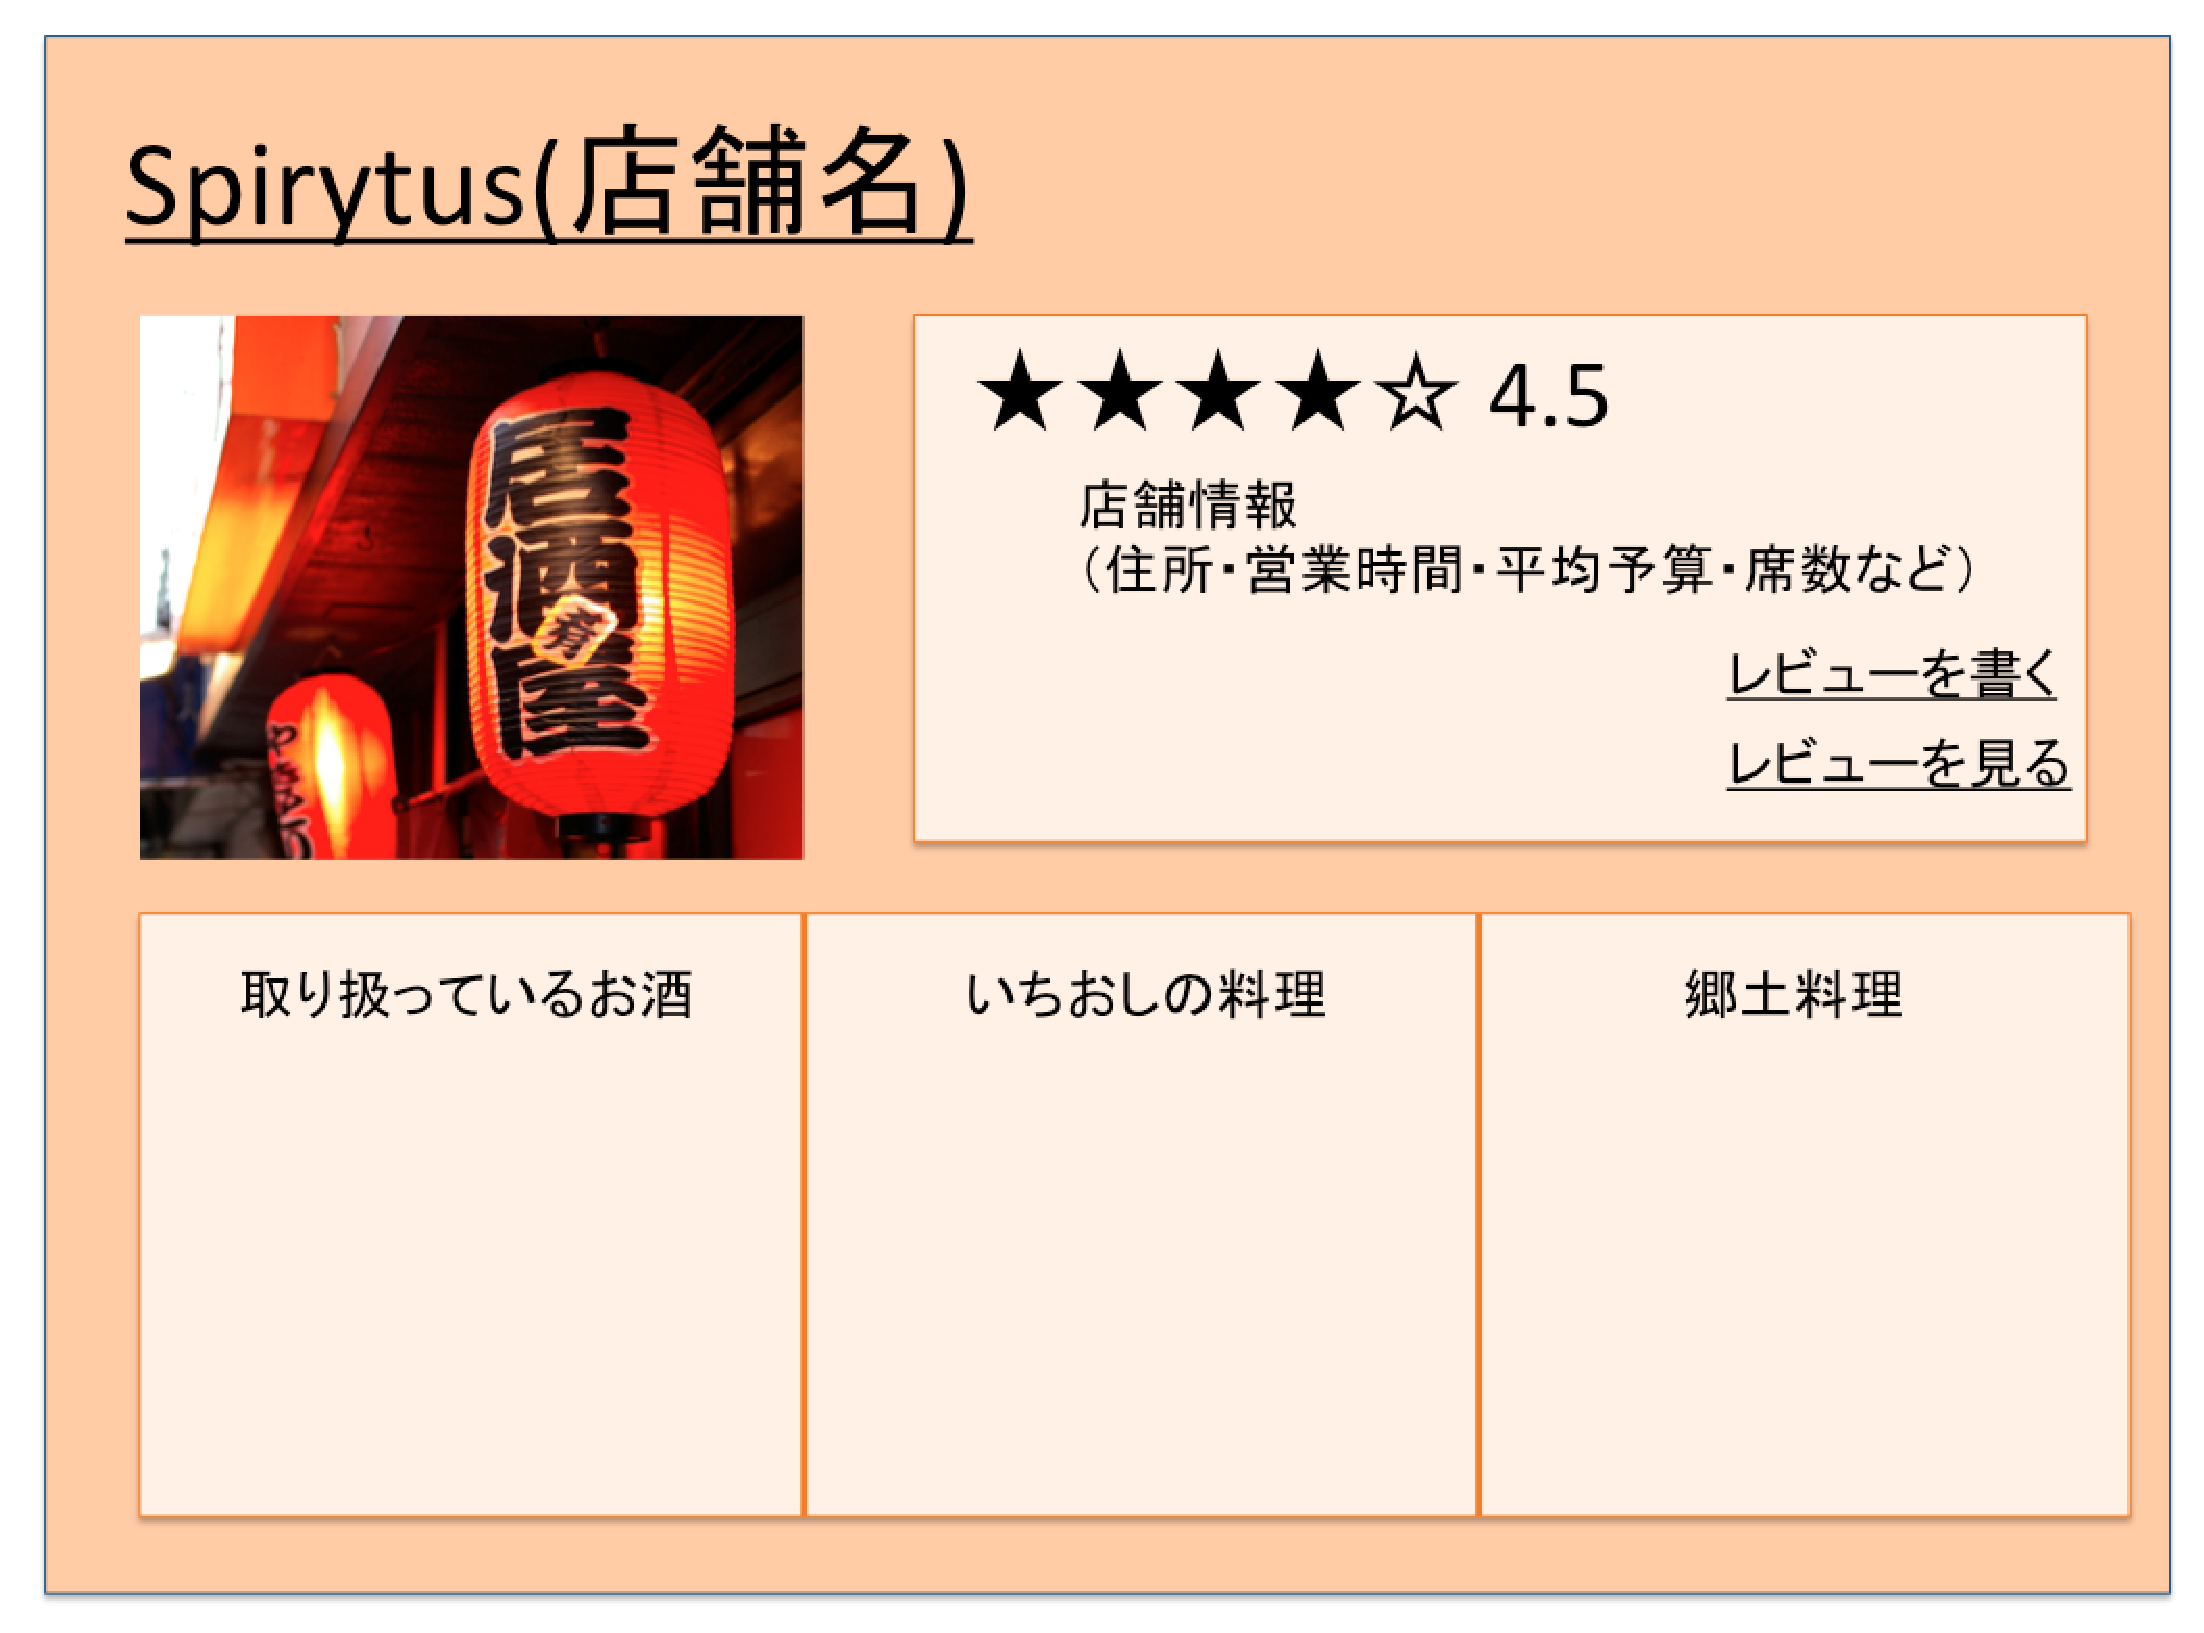
\includegraphics [height=7cm, width=7cm]{extrnal_design_document_image/17.eps}
    \caption {店舗の詳細情報が表示される画面}
    \label {fig:17}
    \end{center}
\end {figure}

\subsection{店舗側の店舗情報登録機能}
店舗情報内容
\begin{enumerate}
\item 店舗名
\item 店舗の画像
\item 営業時間(営業日の営業時間や定休日)
\item 店舗の位置(店舗の住所)
\item 交通手段(最寄の駅から車・徒歩等での所要時間)
\item 店舗の予約用電話番号(電話の際の注意事項も付け加える)
\item 座席数(個室数、カウンター数、宴会場の収容人数)
\item 喫煙席の有無
\item コースメニューの内容と値段
\item 店舗のHPやブログのURL
\item メニューと価格(お勧めだけでも)
\item 店のアピール
\end{enumerate}

店舗情報の登録機能では上記のような店側が店舗の決められている営業時間や全体のメニュー、その他の情報を登録する機能です。
\section{データ定義}
本章では、データベースで管理するデータについて定義します。
データベースのテーブルは、表\ref{tables}に示すテーブル群から構成されます。
また、これらのテーブル間のつながりを示したER図を別添ファイル「ER図.pdf」に、
各テーブルの定義を別添ファイル「データ定義書.pdf」に示します。
​
\begin{table}[!htbp]
\caption{データテーブル一覧}
\label{tables}
\begin{center}
\begin{tabular}{|l|l|l|}\hline
テーブル名 & 内容 & 詳細\\\hline\hline
liquors & お酒 & お酒に関する情報\\\hline
stores & 店舗 & 店舗に関する情報\\\hline
dishes & 料理 & 料理に関する情報\\\hline
ingredients & 食材 & 食材に関する情報\\\hline
resorts & 観光地 & 観光地に関する情報\\\hline
alcoholics & 酒類 & 酒類に関する情報\\\hline
brewers & 酒造 & 酒造に関する情報\\\hline
liquor\_reviews & お酒のレビュー & お酒のレビューに関する情報\\\hline
store\_reviews & 店舗のレビュー & 店舗のレビューに関する情報\\\hline
users & ユーザ & ユーザに関する情報\\\hline
store\_liquors & 店舗にあるお酒 & 店舗とお酒を関連付ける情報\\\hline
store\_dishes & 店舗にある料理 & 店舗と料理を関連付ける情報\\\hline
desh\_ingredients & 料理の食材 & 料理と食材を関連付ける情報\\\hline
\end{tabular}
\end{center}
\end{table}

\section{ネットワーク設計}
本システムは図\ref{net}のようにHTTPを用いてクライアントとサーバのやり取りを行います。
\begin{enumerate}
  \item クライアント側がサーバ側に「リクエスト」を送信します
  \item サーバ側でリクエストの解析・処理してリクエストの答えを作ります
  \item サーバ側がクライアント側に「レスポンス」を返します
\end{enumerate}
\begin{figure}[h]
  \begin{center}
    \includegraphics[width=0.8\linewidth]{net.eps}
    \caption{クライアントとサーバのやり取り}
    \label{net}
  \end{center}
\end{figure}

図\ref{server}のようにサーバを多重化することで片方のサーバに障害が発生した場合でも、もう片方のサーバでサービスを運用することが可能です。さらにデータベースのバックアップを行うことでデータの損失を防ぎます。
\begin{figure}[h]
  \begin{center}
    \includegraphics[width=0.8\linewidth]{server.eps}
    \caption{サーバの中について}
    \label{server}
  \end{center}
\end{figure}


\section{セキュリティ対策}
\subsection{不正アクセス対策}
ファイアウォールの導入により、不正アクセスが行われることを防ぎます。
また、侵入検知システム(IDS)を導入することで、
不正アクセスの兆候を検知し、早めの対応を行えるようにします。
\subsection{暗号化通信}
サーバ・クライアント間の通信は全てSSL通信を利用します。
これにより、通信内容の盗聴されることで情報が外部に漏洩することを防ぎます。
また、ユーザからの信頼性を向上させるために、SSL証明書を購入およびインストールします。
\subsection{ユーザ認証}
このシステムでは、店舗情報の登録および更新やユーザによるレビュー投稿機能を、
その権限のないユーザが行うことを防ぐために、ユーザ認証を行います。
店舗関係者とユーザのログイン時は、登録されたe-mailアドレスとパスワードの組み合わせにより認証を行います。
また、パスワードをハッシュ化してからデータベースに保存することで、
データベース内の情報が外部に漏洩してもパスワードが第三者に知られることを防ぎます。

\section{障害対策}
\subsection{ソフトウェアの障害対策}
データベースの障害対策として、メインで使用するHDD以外のHDDに、
データベースのバックアップを保存します。
毎日深夜0時に自動でバックアップを行い、
障害発生時にはこのバックアップデータからリストアし、復元します。
\subsection{許容停止時間}
障害発生によりシステムが機能しない場合、
直ちに再稼働のための手続きを行います。
システムが停止してから再稼働までの許容停止時間は48時間とします。

\section{ソフトウェア品質}
システムに組み込むプログラムは全て、テストを通過したもののみを扱います。
これにより常に一定の品質を確保します。
システムにバグが発見された場合には、直ちに修正しシステムをアップデートし、
必要に応じてテストの内容を更新します。




\end{document}
